\documentclass[11pt,a4paper]{article}	% Define document class

\usepackage[utf8]{inputenc}				%! Character encoding
\usepackage[T1]{fontenc}					%! Font encoding
\usepackage[english]{babel}				%! Language setting
\usepackage[margin=2.5cm]{geometry}		% Margin size
\usepackage{enumerate}					% Custom enumeration lists
\usepackage[stable]{footmisc}			% Stable footnotes in headings
\usepackage{natbib}						% Bibliography
\usepackage{float}						% Figure floats
\usepackage{multirow}					% Merge rows
\usepackage{hyperref}					% Hyperreferences
\hypersetup{								% Setup of hyperref
	colorlinks,
	citecolor=black,
	filecolor=black,
	linkcolor=black,
	urlcolor=blue
}

\usepackage{amsmath}					% AMS math
\usepackage{amssymb}						% Math symbols
\usepackage{amsthm}						% Custom theorem environments
\usepackage{units}						% Numerical fractions
\usepackage{subfig}						% Subfigures
\usepackage{tikz}						% TikZ graphics
\usepackage{pgfplots}					% PGFPlots

% Cartesian style definition
\pgfplotsset{
	cartesian/.style={
		% Axis alignment
		axis x line=middle,
		axis y line=middle,
		% Axis label alignment
		every axis x label/.style={at={(current axis.right of origin)},anchor=north west},
		every axis y label/.style={at={(current axis.above origin)},anchor=north east},
		% Legend alignment
		every axis legend/.append style={legend pos=outer north east}
		},
	compat=1.8			% Version declaration for compatibility
}

% Custom theorems
\newtheorem{theorem}{Theorem}[]
\newtheorem{problem}{Problem}
\theoremstyle{remark}
\newtheorem{corollary}[theorem]{Corollary}

\DeclareMathOperator*{\plim}{plim}

\title{\LaTeX\ for Economists -- Mini exam}
\author{Attila Gyetvai}
\date{}									% Leave empty for no date

%%%%%%%%%%%%%%%%%%%%%%%%%%%%%%%%%

\begin{document}

\maketitle

\begin{abstract}
	This is the mini exam for the \LaTeX\ for Economists course at CEU.
\end{abstract}

\tableofcontents
\listoffigures
\listoftables

\section{Topics\footnote{A footnote in headings is not straightforward.}}

\begin{enumerate}[(a)]
	\item
	Text styling
	\begin{enumerate}[(i)]
		\item
		Bold, emphasize
		\item
		Alignment, spacing
	\end{enumerate}
	\item
	Math
	\item
	Graphics
\end{enumerate}

If stuck, refer to \href{http://google.com}{Google}.

\section{Math}

\begin{problem}[Wooldridge Problem 9.7 (i)]
(This problem is taken from \cite{wldr}.)

Consider the simple regression model with classical measurement error, $y = \beta_0 + \beta_1 \, x^* + u$, where we have $m$ measures on $x^*$.
Write these as $z_h = x^* + e_h, h = 1, \ldots , m$.
Assume that $x^*$ is uncorrelated with $u, e_1 , \ldots , e_m$, that the measurement errors are pairwise uncorrelated, and have the same variance, $\sigma_e^2$.
Let $w = (z_1 + \ldots + z_m)/m$ be the average of the measures on $x^*$, so that, for each observation $i$, $w_i = (z_{i1} + \ldots + z_{im})/m$ is the average of the $m$ measures.
Let $\bar{\beta}_1$ be the OLS estimator from the simple regression $y_i$ on $1, w_i , i = 1, \ldots , n$, using a random sample of data.
Show that
\begin{equation}
	\plim_{n \to \infty} (\bar{\beta}_1) = \beta_1 \cdot \left\lbrace \frac{\sigma_{x^*}^2}{\sigma_{x^*}^2 + \frac{\sigma_e^2}{m}} \right\rbrace .
\end{equation}

\end{problem}

The meaning of matrix $X$ can be found in Table \ref{tab:x}.

\begin{table}[H]
	\centering
	\begin{tabular}{|c|c|}
		\hline
		\textbf{Notation} & \emph{Meaning} \\
		\hline
		$X$ & $\begin{pmatrix}
			x_{11} & x_{12} & \ldots & x_{1n} \\
			x_{21} & x_{22} & \ldots & x_{2n} \\
			\vdots & \vdots & \ddots & \vdots \\
			x_{m1} & x_{m2} & \ldots & x_{mn}
		\end{pmatrix}$ \\
		\hline
		\multicolumn{2}{|c|}{An $m \times n$ matrix} \\
		\hline
	\end{tabular}
	\caption{What does $X$ mean?}
	\label{tab:x}
\end{table}

\newpage

\section{Graphics}

This section include figures \ref{fig:square} and \ref{fig:plots}.
Figure \ref{fig:plots} consists of figures \ref{fig:2d} and \ref{fig:3d}.

\begin{figure}[H]
	\centering
	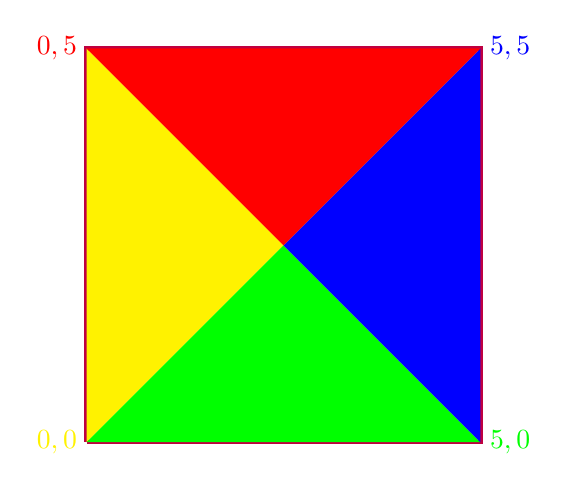
\begin{tikzpicture}
		\draw [purple, ultra thick] (0,0) coordinate (a) -- (5,0) coordinate (b) -- (5,5) coordinate (c) -- (0,5) coordinate (d) -- (a);
		\fill [yellow] (a) -- (2.5,2.5) coordinate (e) -- (d);
		\fill [green] (a) -- (b) -- (e);
		\fill [blue] (b) -- (c) -- (e);
		\fill [red] (c) -- (d) -- (e);
		\node [left, yellow] at (a) {$0,0$};
		\node [right, green] at (b) {$5,0$};
		\node [right, blue]  at (c) {$5,5$};
		\node [left, red]    at (d) {$0,5$};
	\end{tikzpicture}
	\caption{A colorful square.}
	\label{fig:square}
\end{figure}

\begin{figure}[H]
	\centering
	\subfloat[2D plot.]{
	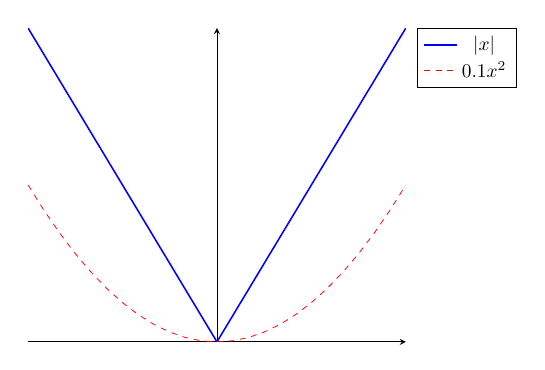
\begin{tikzpicture}[scale=0.7]
		\begin{axis}[
			cartesian,
			ticks=none
		]
			\addplot [blue, thick] {abs(x)};
			\addplot [red, dashed] {0.1*x^2};
			\legend {$|x|$, $0.1 x^2$};
		\end{axis}
	\end{tikzpicture}
	\label{fig:2d}}
	\hspace*{2em}
	\subfloat[3D plot (mesh).]{
	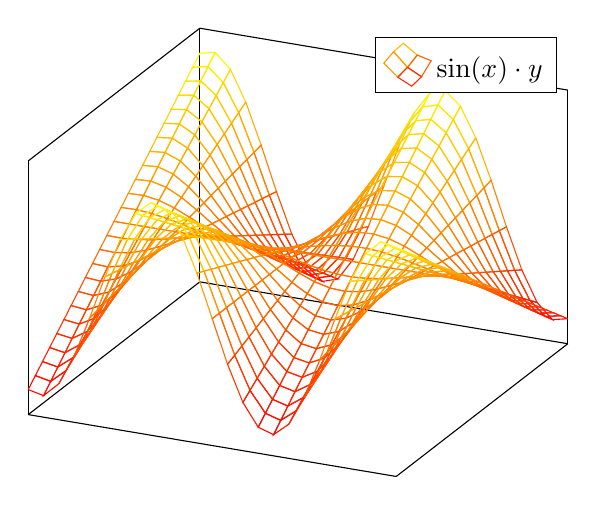
\begin{tikzpicture}
		\begin{axis}[
			colormap/redyellow,
			ticks=none
		]
			\addplot3 [mesh] {sin(deg(x))*y};
			\legend {$\sin (x) \cdot y$};
		\end{axis}
	\end{tikzpicture}
	\label{fig:3d}}
	\caption{2- and 3-dimensional plots.}
	\label{fig:plots}
\end{figure}

\bibliographystyle{apalike}
\bibliography{mybib}

\end{document}
